\documentclass[]{standalone}
%\input{packages_settings}

\usepackage{pgfplots}

\pgfplotsset{width=7cm,compat=1.8}
\begin{document}
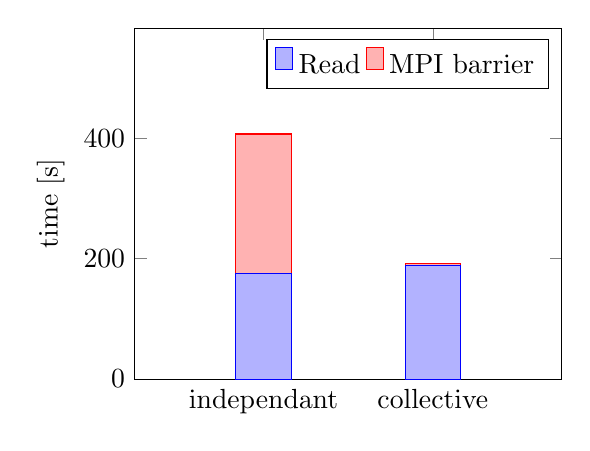
\begin{tikzpicture}
\begin{axis}[
    ybar stacked,
	bar width=20pt,
	%nodes near coords,
    enlargelimits=0.76,
    legend pos = north east,
    legend style={legend columns=-1},
    ylabel={time [s]},
    symbolic x coords={independant, collective},
    xtick=data,
    %x tick label style={rotate=45,anchor=east},
    ]
\addplot+[ybar] plot coordinates {(independant,175.6738287103) (collective,188.5937377118)};
\addplot+[ybar] plot coordinates {(independant,231.2120801987) (collective,2.6859489382)};
\legend{\strut Read, \strut MPI barrier}
\end{axis}
\end{tikzpicture}
\end{document}
